\chapter{Completitud}

Una propiedad importante de los espacios m\'etricos es la
completitud. En esta unidad introducimos esta propiedad e
indagamos algunas de sus consecuencias.
\section{Sucesiones}
\begin{definicion} Una \index{\emph{sucesi\'on}} en un e.m. $(X,d)$ es una
funci\'on $f:\nn\rightarrow X$.
\end{definicion}

Esta el la definici\'on formal de sucesi\'on, no obstante cuando
se trabaja con sucesiones no se hace alusi\'on expl\'{\i}cita a la
funci\'on $f$ de la definici\'on. Normalmente una sucesi\'on se
introduce con el s\'{\i}mbolo $\{a_n\}_{n\in\nn}$ o, brevemente,
$\{a_n\}$, asumiendo que los \'{\i}ndices $n$ son naturales. Claro
est\'a que, \'{\i}mplicitamente, estos s\'{\i}mbolos conllevan la
funci\'on $f$. Esta es la funci\'on tal que $f(n)=a_n$.

\begin{definicion}\label{def,sucesionconvergente} Sea $\{a_n\}$ una sucesi\'on en el e.m.
$(X,d)$. Diremos que esta sucesi\'on \emph{converge} al punto
$a\in X$ (denotaremos esto por $a_n\rightarrow a$) si, y solo si,
para todo entorno $U$ de $a$ existe un $n_0=n_0(U)$ tal que cuando
$n\geq n_0$ se tiene que $a_n\in U$. Sinteticamente, dado
cualquier entorno, salvo posiblemente una cantidad finita de
t\'erminos de la sucesi\'on todos los t\'erminos restantes est\'an
inclu\'{\i}dos en el entorno, ver la Figura
\vref{fig,sucesionconvergente}
\end{definicion}

\begin{figure}
\begin{center}
    \psfrag{a}{$a$}
    \psfrag{a1}{$a_1$}
    \psfrag{a2}{$a_2$}
    \psfrag{an}{$a_{n_0}$}
    \psfrag{an1}{$a_{n_0+1}$}
    \includegraphics[height=5cm, width=7cm]{succonv.eps}
    \caption{ Definici\'on
    \vref{def,sucesionconvergente}}\label{fig,sucesionconvergente}
\end{center}
\end{figure}

La convergencia es una propiedad topol\'ogica. Confiamos en que el
alumno tiene muchos ejemplos de sucesiones convergentes en $\rr$,
esto fu\'e visto en C\'alculo I. Vamos a ver que sucede en otros
espacios m\'etricos.

\begin{ejemplo} En un e.m. discreto $(X,d)$ si una sucesi\'on
$\{a_n\}$  converge al punto $a$, entonces a partir de un $n_0$ en
adelante se tiene que $a_n=a_{n_0}$. En efecto, esto es
consecuencia de considerar el siguiente entorno:
$U=B(a,1/2)=\{a\}$.
\end{ejemplo}

\begin{ejemplo}\label{ejem,convfunciones} Consideremos el e.m. $(C([0,1]),d)$, donde
$C([0,1])$ representa al conjunto de funciones continuas
$f:[0,1]\rightarrow\rr$ y $d$ es la m\'etrica definida en el
Ejemplo \vref{ejem,distsobrecontl1}. Consideremos las funciones
definidas por:

\[
    f(x)=\left\{%
\begin{array}{ll}
    nx, & \hbox{si $0\leq x\leq \frac1n$;} \\
    2-nx, & \hbox{si $\frac1n\leq x\leq \frac2n$.} \\
    0,    &\hbox{si $\frac2n\leq x\leq 1.$}
\end{array}%
\right.
\]
En la Figura \vref{fig,convfunciones}, se pueden observar los
gr\'aficos de estas funciones.
\begin{figure}
\begin{center}
    \psfrag{f1}{$f_1$}
    \psfrag{f2}{$f_2$}
    \psfrag{f3}{$f_3$}
    \psfrag{f4}{$f_4$}
    \psfrag{f5}{$f_5$}
    \psfrag{f6}{$f_6$}
    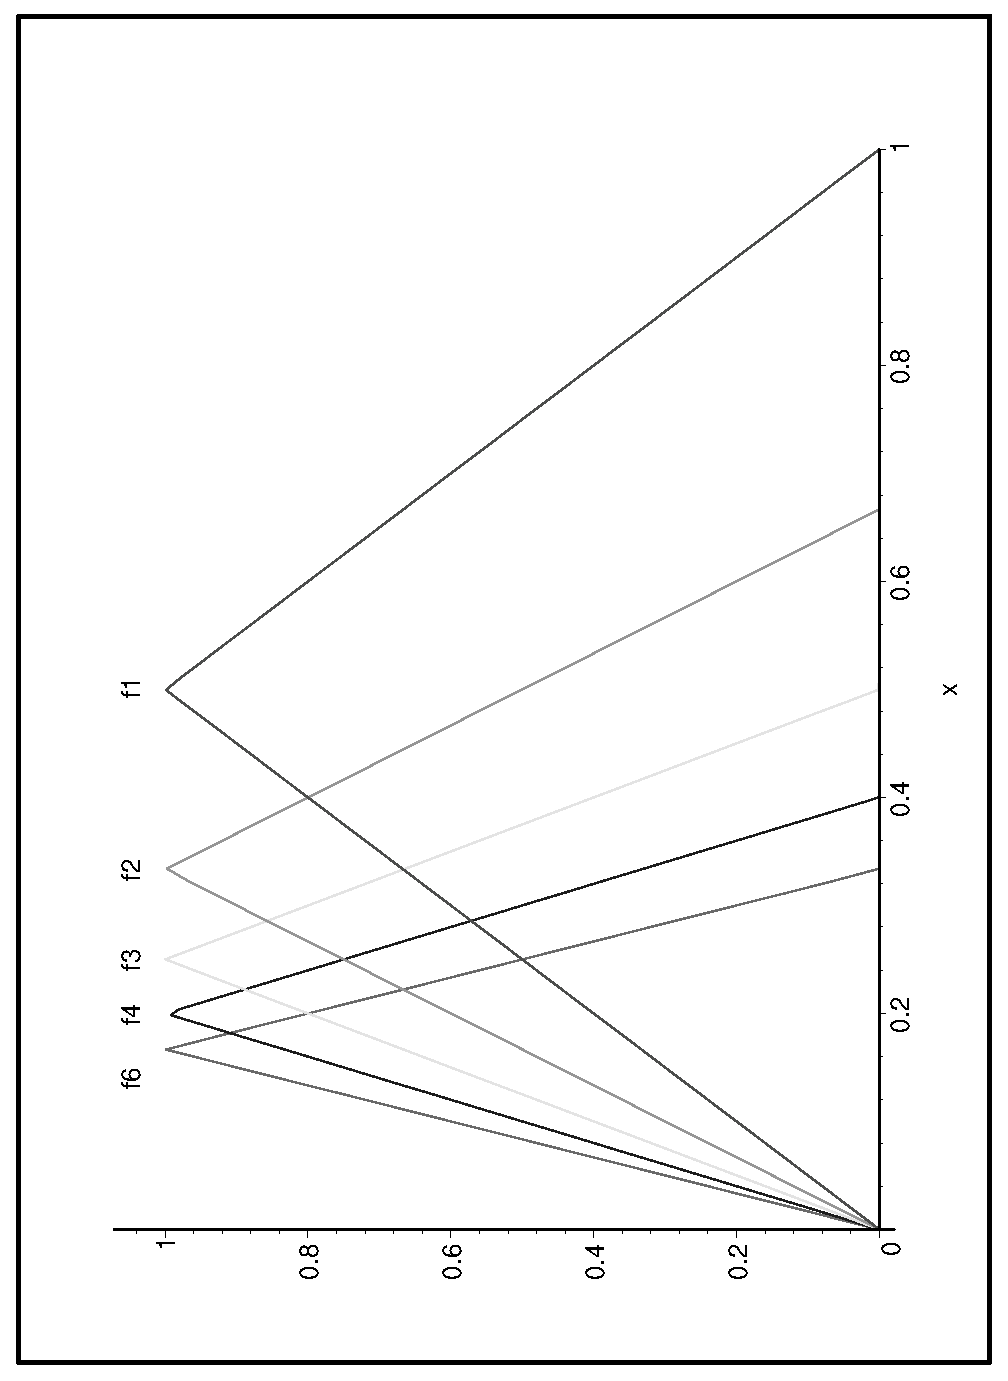
\includegraphics[height=12cm, width=7cm, angle=-90]{funciones0.eps}
    \caption{Funciones del Ejemplo
    \ref{ejem,convfunciones}}\label{fig,convfunciones}
\end{center}
\end{figure}
Es un ejercicio de C\'alculo I demostrar que $f_n\rightarrow 0$
con la m\'etrica propuesta. Sin embargo, sobre $C([0,1])$ tenemos
definida otra m\'etrica, a saber: la del Ejemplo
\vref{ejem,distsobrecont}. Con esta m\'etrica la sucesi\'on $f_n$
no converge a ninguna funci\'on.
\end{ejemplo}

Es posible caracterizar algunos de los conceptos, que ya hemos
visto, en t\'erminos de sucesiones. Por ejemplo, el concepto de
clausura y continuidad.

\begin{proposicion} Sea $(X,d)$ un e.m. y $A\subset X$. Entonces
$a\in\C{A}$ si, y solo si, existe una sucesion $a_n\in A$ tal que
$a_n\rightarrow a$.
\end{proposicion}
\begin{demo} Supongamos que $a\in\C{A}$, entonces, para todo
$n\in\nn$ se tiene que $B(a,1/n)\cap A\neq\emptyset$. Sea, pues,
$a_n\in B(a,1/n)\cap A$. Se puede ver, sin dificultad, que
$a_n\rightarrow a$. Rec\'{\i}procamente, supongamos que existe la
sucesi\'on $\{a_n\}$. Si $U$ es un entorno arbitrario de $a$,
entonces, puesto que $a\in\C{A}$, tenemos que, para ciertos $n$,
$a_n\in U$, luego, estos $a_n$, estan en la intersecci\'on de $U$
con $A$, lo que implica que esta es no vac\'{\i}a. Eso prueba que
$a\in\C{A}$.
\end{demo}

\section{Sucesiones de Cauchy, espacios m\'etricos completos}


\begin{definicion}
\begin{itemize}
\item[i)]Dada una sucesi\'on $\{a_n\}$ en un e.m. $(X,d)$, diremos que
$\{a_n\}$ es una \emph{sucesi\'on de Cauchy} si: para todo
$\epsilon>0$ existe un $n_0=n_0(\epsilon)$\footnote{Con
$n_0=n_0(\epsilon)$ queremos decir que el n\'umero $n_0$ depende
de $\epsilon$ pero que normalmente no usaremos la notaci\'on
$n_0(\epsilon)$ sino, simplemente, $n_0$} tal que para $n,m\geq
n_0$ tenemos que $d(a_n,a_m)<\epsilon$. En otras palabras, para
valores grandes de $n$ los t\'erminos $a_n$ est\'an cerca entre
si.
\item[ii)] Un e.m. se dir\'a \emph{completo} si, y solo si, todo
sucesi\'on de Cauchy en \'el es convergente.
\end{itemize}
\end{definicion}


Como acabamos de decir, en un e.m. completo toda sucesi\'on de
Cauchy converge. La reciproca de esta afirmaci\'on es siempre
cierta, es decir en cualquier e.m. toda sucesi\'on convergente es
de Cauchy. En efecto, sea $\{a_n\}$ una sucesi\'on convergente en
$(X,d)$ al punto $a$ y sea  $\epsilon > 0$. Existe un
$N=N(\epsilon)$ tal que para $n>N$ se tiene que
\[
    d(a_n,a)<\frac{\epsilon}{2}.
\]
Luego, para $n,m>N$ y por la desigualdad tri\'agular, tenemos que
\[
    d(a_n,a_m)\leq d(a_n,a)+d(a,a_m)<\frac{\epsilon}{2}+\frac{\epsilon}{2}=\epsilon.
\]
Esto prueba que la sucesi\'on es de Cauchy, como quer\'{\i}amos.

Un ejemplo importante de e.m. completo es $\rr$. Esta propiedad de
$\rr$ es enunciada, pr\'acticamente, como un axi\'oma. Hablaremos,
mas no sea brevemente, de los ``fundamentos'' de los
 n\'umeros reales en el ap\'endice al final de esta unidad, ver
 Secci\'on  \vref{sec,apendice}. Sabiendo que $\rr$ con la
 m\'etrica del m\'odulo es completo podemos demostrar la
 completitud de otros e.m., como veremos m\'as abajo. Antes de ver
 esto demostremos que toda sucesi\'on convergente es de Cauchy

 \begin{ejemplo} $\rr^n$ con la m\'etrica euclidea es un e.m.
 completo.\footnote{Observar que, en virtud del Ejercicio
 \vref{ejer,completitudconmetequi} $\rr^n$ con cualquier
 m\'etrica equivalente a la euclidea tambi\'en resultar\'a
 completo} Vamos a demostrar esta afirmaci\'on. Denotemos
 por letras en negritas $\mathbf{x}$, $\mathbf{y}$, $\mathbf{z}$,
 etc $n$-uplas en $\rr^n$, es decir $\mathbf{x}=(x_1,\dots, x_n)$
 con $x_i\in\rr$, $i=1,\dots,n$. Consideremos una sucesi\'on de
 Cauchy  $\{\mathbf{x}_j\}_{j\in\nn}$ en $\rr^n$. Esto nos determina $n$
 sucesiones en $\rr$, puesto que
 $\mathbf{x}_j=(x_1^j,\dots,x_n^j)$. Veamos que, para cada $i$,
 $\{x_i^j\}_{j\in\nn}$ es una sucesi\'on de Cauchy en $\rr$. Se
 tiene que:
\[
    |x_i^j-x_i^k|\leq \sqrt{\sum\limits_{s=1}^n(x_s^j-x_s^k)^2}\leq
    d(\mathbf{x}_j,\mathbf{x}_k).
\]
Como el \'ultimo miembro se puede hacer tan chico como queramos,
puesto que $\{\mathbf{x}_j\}$ es de Cauchy, podemos conseguir lo
mismo para el primer miembro, esto es $\{x_i^j\}$ es de Cauchy.
As\'{\i}, como $\rr$ es completo, existe un $x_i$, para
$i=1,\dots,n$ tal que $x_i^j\rightarrow x_i$, para
$j\rightarrow\infty$. Definamos, pues,
$\mathbf{x}=(x_1,\dots,x_n)$ y veamos que $\mathbf{x}_j\rightarrow
\mathbf{x}$. Sea $\epsilon>0$, para cada $i=1,\dots,n$ podemos
hallar un $j(\epsilon,i)$, es decir $j$ depende de $\epsilon $ y
de $i$, tal que para $j\geq j(\epsilon, i)$ tenemos que:
\[
    |x_i^j-x_i|<\frac{\epsilon}{\sqrt{n}}.
\]
As\'{\i}, si:
\[
    j\geq\max\limits_{1\leq i\leq n}j(\epsilon,i)
\]
entonces
\[
    d(\mathbf{x}_j-\mathbf{x})=\sqrt{\sum\limits_{i=1}^n(x_i^j-x_i)^2}=
    \sqrt{\sum\limits_{i=1}^n\frac{\epsilon^2}{n}}=\epsilon,
\]
lo que demuestra que $\mathbf{x}_j\rightarrow \mathbf{x}$, como
quer\'{\i}amos.
\end{ejemplo}

\begin{ejemplo}\label{ejem,emnocompleto} El e.m. $(C([0,1]),d)$, con $d$ como en el Ejemplo
\vref{ejem,convfunciones}, no es completo. Consideremos las
siguientes funciones, para $n/geq 2$:

\[
    f_n(x):=\left\{
                \begin{array}{ll}
                        1, & \hbox{si $0\leq x\leq \frac12$;} \\
                        -nx+\frac{n+2}{2n}, & \hbox{si $\frac12\leq x\leq \frac12+\frac1{n}$;} \\
                        0, & \hbox{si $\frac12\leq x\leq 1$.} \\
\end{array}
\right.
\]
 en la Figura \vref{fig,emnocompleto} graficamos estas
funciones.
\begin{figure}[h]
\begin{center}
    \psfrag{f2}{$f_2$}
    \psfrag{f3}{$f_3$}
    \psfrag{f4}{$f_4$}
    \psfrag{f5}{$f_5$}
    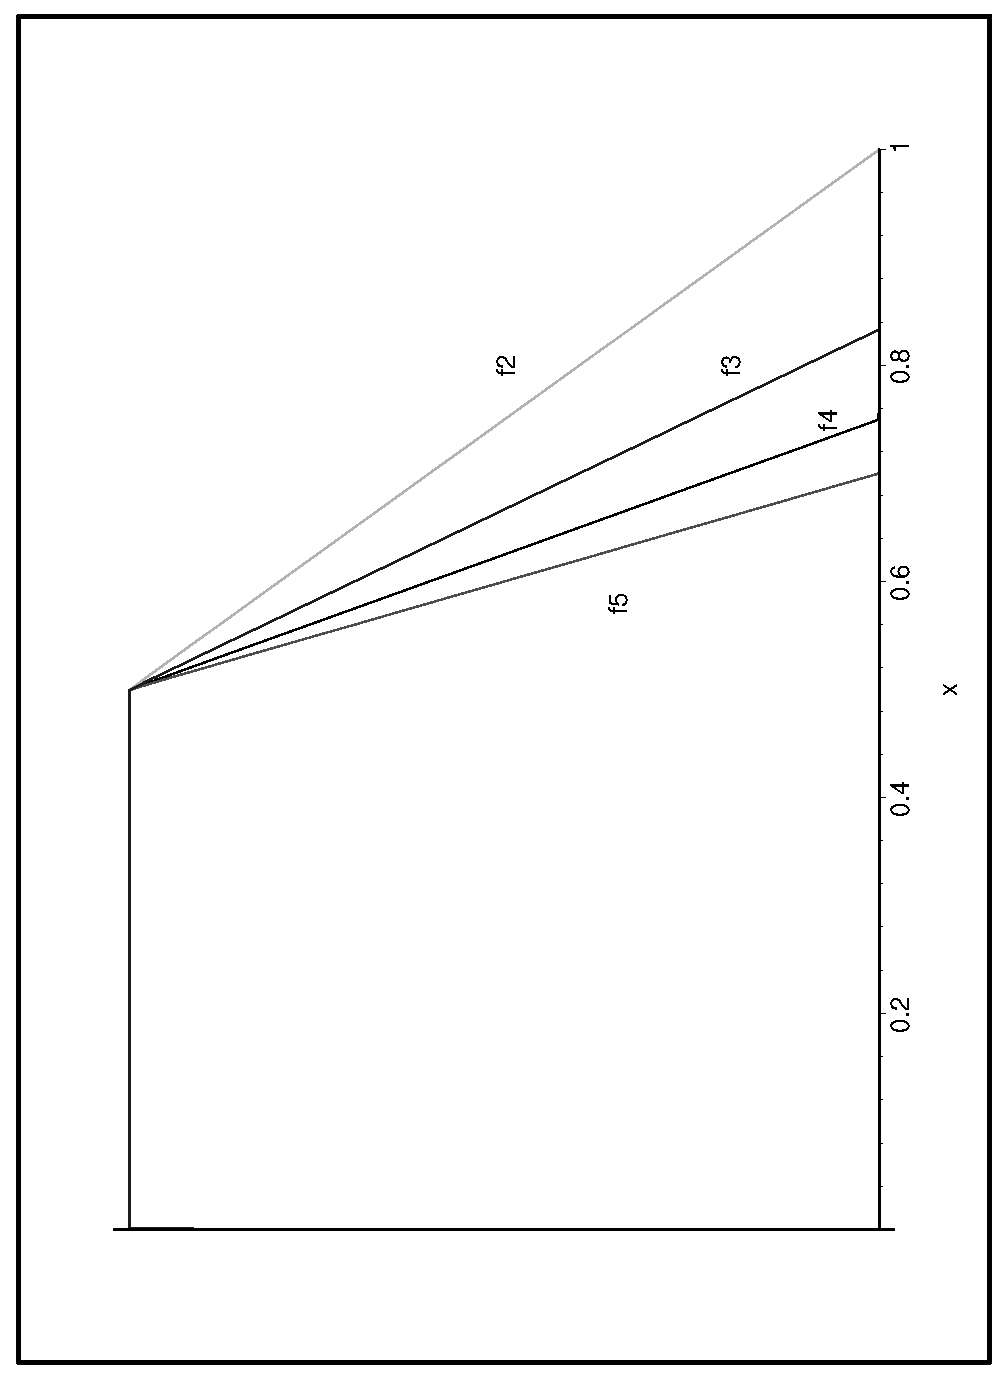
\includegraphics[height=12cm,width=7cm,angle=-90]{funciones1.eps}
    \caption{Funciones del Ejemplo
    \ref{ejem,emnocompleto}}\label{fig,emnocompleto}
\end{center}
\end{figure}

No es dificil convencerse que esta es una sucesi/'on de Cauchy,
puesto que, para $j,k/geq n$ tenemos que:

\[
    d(f_j,f_k)=\frac12|\frac1j-\frac1k|\leq \frac1n\rightarrow
    0\quad\text{cuando}\quad n\rightarrow \infty.
\]
Sin embargo estas funciones no convergen a ninguna funci\'on en
$C([0,1])$. Para ver esto, supongamos que, por el contrario,
existe $f\in C([0,1])$ tal que $f_n\rightarrow f$. Vamos a
demostrar que, necesariamente, $f$ debe valer 1 en el intervalo
$[0,1/2)$ y debe valer 0 en el intervalo $(1/2,1)$, por tal motivo
no podr\'{\i}a ser continua contradiciendo las hip\'otesis. Vamos
a demostrar solo que $f$ es 0 en $(1/2,1)$, la otra parte es
similar y aun m\'as facil. Supongamos que exista $1/2<a<1$ tal que
$f(a)\neq 0$, podemos suponer que $f(a)>0$. Elijamos $\delta_1>0$
suficientemente peque\~no de modo que $1/2<a-\delta_1$ y elijamos
$\delta_2>0$ suficientemente peque\~no de modo tal que
$f(x)>f(a)/2$ para $x\in(a-\delta_2,a+\delta+2)$ (esto es posible
pues $f$ es continua en $a$). Ahora, el n\'umero
$\delta:=\min\{\delta_1,\delta_2\}$ satisface las dos propiedades
anteriores simultaneamente. Podemos encontrar un $n_0$
suficientemente grande para que $1/2+1/n<a-\delta$, cuando
$n>n_0$, esto implica que $f_n$ es id\'enticamente cero en el
intervalo $(a-\delta,a+\delta)$, ver la Figura
\vref{fig,dememnocompleto}.
\begin{figure}[h]
\begin{center}
    \psfrag{a}{$a$}
    \psfrag{a-d}{$a-\delta$}
    \psfrag{a+d}{$a+\delta$}
    \psfrag{fa}{$f(a)$}
    \psfrag{fa2}{$\frac{f(a)}{2}$}
    \psfrag{f}{$f$}
    \psfrag{com}{El \'area del rect\'agulo es $\delta f(a)$}
    \includegraphics[height=8cm,width=12cm]{demnoco.eps}
    \caption{Construcci\'on de la demostraci\'on en el Ejemplo
    \ref{ejem,emnocompleto}}\label{fig,dememnocompleto}
\end{center}
\end{figure}
Juntando todas las propiedades vistas en el p\'arrafo anterior,
deducimos que, para $n>n_0$,
\[
    d(f_n,f)=\int_0^1|f_n-f|dx\geq\int_{a-\delta}^{a+\delta}|f_n-f|dx\geq
    \delta f(a)>0.
\]
De modo que $f_n$ no converge a $f$, contradiciendo nuestras
suposiciones.
\end{ejemplo}


Ahora veremos que subespacios, de un e.m. completo, son, a su vez,
completos.

\begin{proposicion} Sea $(X,d)$ un e.m. completo e $Y\subset X$.
Son equivalentes:
\begin{itemize}
\item[i)] $(Y,d)$ es un subespacio completo.
\item[ii)] $Y$ es cerrado en $X$.
\end{itemize}
\end{proposicion}



\section{Ap\'endice}\label{sec,apendice}
 Hay dos \'opticas para introducir los numeros
 reales, las denominaremos axiom\'atica y constructiva.
 Describimos a continuaci\'on, y someramente, cada una de ellas.

 Se pueden introducir los n\'umeros reales a travez de un sistema
 axiom\'atico. Como es conocido, un sistema axiom\'atico consta de
 \emph{t\'erminos primitivos}, que son, por decirlo as\'{\i}, los
 objetos iniciales, a travez de los cuales se construyen todos los
 dem\'as objetos de la teor\'{\i}a. Pueden ser t\'erminos
 primitivos: conjuntos, operaciones, relaciones, etc. Es importante
 aclarar que los t\'erminos primitivos son objetos puramente
 hipot\'eticos, es decir no se afirma la existencia de estos
 objetos. Los t\'erminos primitivos para los n\'umeros reales son:
 un conjunto, comunmente denotado por $\rr$, dos funciones de
  $\rr\times\rr$ en $\rr$, usualmente denotadas por $+$ y $.$\footnote
  {Estas operaciones se denominan suma y multiplicaci\'on,
  usualmente se omite el signo de multiplicaci\'on} y una relaci\'on
  $\leq$. Para completar el sistema axiom\'atico,
  debemos dar los axiomas, estos son propiedades que se postulan
  para los t\'erminos primitivos. Los axiomas para los n\'umeros
  reales los podemos dividir en cuatro grupos:

  \begin{itemize}
    \item[1)] $\rr$ es un cuerpo, es decir:
        \begin{itemize}
            \item[1.1)] $x+(y+z)=(x+y)+z$;
            \item[1.2)] $x+y=y+x$;
            \item[1.3)] Existe un elemento $0\in\rr$ tal que $x+0=x$;
            \item[1.4)] Para cada $x\in\rr$ existe un $y\in\rr$
            tal que $x+y=0$;
            \item[1.5)] $x(yz)=(xy)z$;
            \item[1.6)] $xy=yx$;
            \item[1.7)] Existe un elemento $1\in\rr$ tal que
            $1.x=x$;
            \item[1.8)] Para cada elemento $0\neq x\in\rr$ existe un
            elemento $y\in\rr$ tal que $xy=1$;
            \item[1.9)] $x(y+z)=xy+xz$;
        \end{itemize}
    \item[2)] $\rr$ es un cuerpo ordenado.
        \begin{itemize}
            \item[2.1)] Si $x\leq y$ e $y\leq z$ entonces $x\leq
            z$;
            \item[2.2)] Si $x\leq y$ e $y\leq x$ entonces $x=y$;
            \item[2.3)] Si $x$ e $y$ pertenecen a $\rr$ entonces
            $x\leq y$ o $y\leq x$;
            \item[2.4)] Si $x\leq y$ entonces $x+z\leq y+z$;
            \item[2.5)] Si $0\leq x$ e $0\leq y$ entonces $0\leq
            xy$;
        \end{itemize}

        Dentro de $\rr$  se puede construir un conjunto, denotado
        por $\mathbb{Z}$. que corresponde a los enteros.
    \item[3)] $\rr$ es un cuerpo ordenado y arquimedeano. Esto es:
    para todo $y\geq 0$ y todo $x>0$ existe un entero $n$ tal que
    $nx\geq y$.

    Por \'ultimo tenemos el axioma de completitud. Hay varias
    formulaciones equivalentes para este axioma, ver el Ejercicio
     \vref{ejer,completitud} nosotros elegimos
    la siguiente:

    \item[4)] Todo subconjunto $A\subset\rr$ acotado
    superiormente, tiene supremo, es decir existe un $\alpha\in\rr$
    tal que: 1) $\alpha$ es una cota superior de $A$, esto es $\alpha\geq x$
    para todo $x\in A$ y 2) $\alpha$ es la m\'as chica de las
    cotas superiores, esto es si $\beta$ es cota superior entonces
    $\alpha\leq\beta$. Observar que no es necesario que $\alpha\in
    A$.
  \end{itemize}



  Hay tres propiedades que
  ser\'{\i}an deseables que un sistema axiom\'atico tuviera: 1)
  \emph{coherencia}, es decir que los axiomas no se
  ``contradigan'' 2)\emph{independencia}, entendiendo por esto que
  los axiomas no sean redundantes, es decir que ninguno de ellos
  se obtenga a partir de los dem\'as y 3)
  \emph{completitud}\footnote{No confundir este concepto con el de
  completitud de un e.m.}, esto es que toda afirmaci\'on de la
  teor\'{\i}a o su negaci\'on se pueda deducir.

  Destacamos,
  nuevamente, que los objetos postulados como t\'erminos
  primitivos en el sistema axiomatico y que satisfagan los axiomas
  podr\'{\i}an no existir. En particular esto ocurre si el sistema
  axiom\'atico es contradictorio. Obviamente, en ese caso, nuestro
  s\'{\i}stema axiom\'atico no servir\'{\i}a de mucho. Esto no sucede para el
  s\'{\i}stema de axiomas para los n\'umeros reales. Este
  s\'{\i}stema tiene un modelo, es decir podemos encontrar un
  conjunto $\rr$ y las funciones y relaci\'on postuladas de modo
  tal que se satisfagan todos los axiomas. Esto nos lleva a la otra \'optica de
  introducci\'on de los n\'umeros reales, la que denominamos constructiva. Varios
  modelos fueron propuestos por diversos matem\'aticos, en
  particular Dedekind y Cantor. Estos modelos
  son construidos a partir de los n\'umeros racionales.\footnote{Es bueno
  decir que tambi\'en es posible construir los n\'umeros
  racionales a partir de los naturales y estos a partir de la
  Teor\'{\i}a de Conjuntos; no obstante esto se aparta
  considerablemente de los objetivos de esta materia} A Dedekind
  le debemos el m\'etodo de cortaduras y a Cantor el m\'etodo de
  sucesiones fundamentales de Cauchy.








\section{Ejercicios}

\begin{ejercicio}\label{ejer,testearconv} Consideremos el conjunto $C([0,1])$ donde
tenemos definidas las dos m\'etricas $d_1$ y $d_2$ de los Ejemplos
\vref{convunifmet} y \vref{l1metint} respectivamente. Determinar
si las siguientes sucesiones son convergentes con estas m\'etricas
y si son de Cauchy.
\begin{itemize}
    \item[i)] $f_n(x):=\frac1n\text{sen}(nx)$.
    \item[ii)] $f_n(x):=x^n$.
    \item[iii)]$f_n(x):=nx^n$.
\end{itemize}
\end{ejercicio}
\begin{ejercicio} Con la misma notaci\'on del ejercicio anterior
demostrar que si $f_n\to f$ con la m\'etrica  $d_1$ entonces lo
mismo ocurre con la m\'etrica $d_2$.
\end{ejercicio}

\begin{ejercicio} Sean $(X,d)$ e $(Y,d')$ dos e.m. y $f:X\to Y$ un homeomorfismo.
Demostrar que la sucesi\'on $\{a_n\}$ es convergente en $X$ si, y
solo si, $f(a_n)$ es convergente en $Y$.
\end{ejercicio}



\begin{ejercicio} Sea $(X,d)$ un e.m., $a\in A$ y $A\subset X$. Demostrar
que existe un sucesi\'on $\{a_n\}$, con $a_n\in A$, para todo $n$,
y:
\[\lim\limits_{n\to\infty}d(a,a_n)=d(a,A).\]
\end{ejercicio}

\begin{ejercicio} Sea $A\subset \rr$ un conjunto acotado
superiormente. Demostrar que existe una sucesi\'on $\{a_n\}$, con
$a_n\in A$, para todo $n$, y adem\'as:
\[
    \sup A=\lim\limits_{n\to\infty} a_n.
\]
\end{ejercicio}

\begin{ejercicio} Demostrar que $(C([0,1]),d_1)$, con $d_1$ como
en el Ejercicio \ref{ejer,testearconv}, es un e.m. completo.
\end{ejercicio}

\begin{ejercicio} Demostrar que un e.m. con una cantidad finita de
elementos es completo.
\end{ejercicio}

\begin{ejercicio} Demostrar que una sucesi\'on de Cauchy es
acotada.
\end{ejercicio}

\begin{ejercicio} Sea $\{a_n\}$ una sucesi\'on en un e.m. $(X,d)$,
demostrar que cualquierqa de las dos condiciones implica que
$\{a_n\}$ es de Cauchy.
\begin{itemize}
    \item[i)] $d(a_n,a_{n+1})\leq \alpha^n$, con $0<\alpha<1$.
    \item[ii)] La siguiente serie es convergente:
    \[
        \sum\limits_{n=1}^{\infty}d(a_n,a_{n+1}).
    \]
\end{itemize}
\end{ejercicio}

\begin{ejercicio}\label{ejer,completitudconmetequi} Sean $d$ y $d'$ dos m\'etricas
 uniformemente equivalentes
sobre el mismo espacio $X$. Demostrar que $(X,d)$ es completo si,
y solo si, $(X,d')$ es completo.
\end{ejercicio}

\begin{ejercicio} Sea $f:X\to Y$ una funci\'on uniformemente
continua entre dos e.m.. Demostrar que si $\{a_n\}$ es de Cauchy
en $X$ entonces $\{f(a_n)\}$ es de Cauchy en $Y$. Dar un
contraejemplo a la afirmaci\'on anterior suponiendo, solo, que $f$
es continua. \emph{Ayuda:} Considerar la recta extendida.
\end{ejercicio}


\begin{ejercicio}\label{ejer,completitud} Demostrar que el axioma de completitud de $\rr$
dado, se puede sustitu\'{\i}r por cualquiera de los siguientes:
\begin{itemize}
    \item[i)] Toda sucesi\'on de Cauchy en $\rr$ converge.
    \item[ii)] \emph{Principio de Encajes de Intervalos}. Sea
    $\{I_n\}_{n\in\nn}$ una sucesi\'on de intervalos cerrados
    tales que $I_{n+1}\subset I_n$, para todo $n$, entonces
    $\bigcap_{n\in\nn}I_n\neq\emptyset$.
\end{itemize}
\end{ejercicio}
